\documentclass{ximera}

%\usepackage{todonotes}

\newcommand{\todo}{}

\usepackage{esint} % for \oiint
\ifxake%%https://math.meta.stackexchange.com/questions/9973/how-do-you-render-a-closed-surface-double-integral
\renewcommand{\oiint}{{\large\bigcirc}\kern-1.56em\iint}
\fi


\graphicspath{
  {./}
  {ximeraTutorial/}
  {basicPhilosophy/}
  {functionsOfSeveralVariables/}
  {normalVectors/}
  {lagrangeMultipliers/}
  {vectorFields/}
  {greensTheorem/}
  {shapeOfThingsToCome/}
  {dotProducts/}
  {partialDerivativesAndTheGradientVector/}
  {../productAndQuotientRules/exercises/}
  {../normalVectors/exercisesParametricPlots/}
  {../continuityOfFunctionsOfSeveralVariables/exercises/}
  {../partialDerivativesAndTheGradientVector/exercises/}
  {../directionalDerivativeAndChainRule/exercises/}
  {../commonCoordinates/exercisesCylindricalCoordinates/}
  {../commonCoordinates/exercisesSphericalCoordinates/}
  {../greensTheorem/exercisesCurlAndLineIntegrals/}
  {../greensTheorem/exercisesDivergenceAndLineIntegrals/}
  {../shapeOfThingsToCome/exercisesDivergenceTheorem/}
  {../greensTheorem/}
  {../shapeOfThingsToCome/}
  {../separableDifferentialEquations/exercises/}
  {vectorFields/}
}

\newcommand{\mooculus}{\textsf{\textbf{MOOC}\textnormal{\textsf{ULUS}}}}

\usepackage{tkz-euclide}
\usepackage{tikz}
\usepackage{tikz-cd}
\usetikzlibrary{arrows}
\tikzset{>=stealth,commutative diagrams/.cd,
  arrow style=tikz,diagrams={>=stealth}} %% cool arrow head
\tikzset{shorten <>/.style={ shorten >=#1, shorten <=#1 } } %% allows shorter vectors

\usetikzlibrary{backgrounds} %% for boxes around graphs
\usetikzlibrary{shapes,positioning}  %% Clouds and stars
\usetikzlibrary{matrix} %% for matrix
\usepgfplotslibrary{polar} %% for polar plots
\usepgfplotslibrary{fillbetween} %% to shade area between curves in TikZ
%\usetkzobj{all}
\usepackage[makeroom]{cancel} %% for strike outs
%\usepackage{mathtools} %% for pretty underbrace % Breaks Ximera
%\usepackage{multicol}
\usepackage{pgffor} %% required for integral for loops



%% http://tex.stackexchange.com/questions/66490/drawing-a-tikz-arc-specifying-the-center
%% Draws beach ball
\tikzset{pics/carc/.style args={#1:#2:#3}{code={\draw[pic actions] (#1:#3) arc(#1:#2:#3);}}}



\usepackage{array}
\setlength{\extrarowheight}{+.1cm}
\newdimen\digitwidth
\settowidth\digitwidth{9}
\def\divrule#1#2{
\noalign{\moveright#1\digitwidth
\vbox{\hrule width#2\digitwidth}}}




% \newcommand{\RR}{\mathbb R}
% \newcommand{\R}{\mathbb R}
% \newcommand{\N}{\mathbb N}
% \newcommand{\Z}{\mathbb Z}

\newcommand{\sagemath}{\textsf{SageMath}}


%\renewcommand{\d}{\,d\!}
%\renewcommand{\d}{\mathop{}\!d}
%\newcommand{\dd}[2][]{\frac{\d #1}{\d #2}}
%\newcommand{\pp}[2][]{\frac{\partial #1}{\partial #2}}
% \renewcommand{\l}{\ell}
%\newcommand{\ddx}{\frac{d}{\d x}}

% \newcommand{\zeroOverZero}{\ensuremath{\boldsymbol{\tfrac{0}{0}}}}
%\newcommand{\inftyOverInfty}{\ensuremath{\boldsymbol{\tfrac{\infty}{\infty}}}}
%\newcommand{\zeroOverInfty}{\ensuremath{\boldsymbol{\tfrac{0}{\infty}}}}
%\newcommand{\zeroTimesInfty}{\ensuremath{\small\boldsymbol{0\cdot \infty}}}
%\newcommand{\inftyMinusInfty}{\ensuremath{\small\boldsymbol{\infty - \infty}}}
%\newcommand{\oneToInfty}{\ensuremath{\boldsymbol{1^\infty}}}
%\newcommand{\zeroToZero}{\ensuremath{\boldsymbol{0^0}}}
%\newcommand{\inftyToZero}{\ensuremath{\boldsymbol{\infty^0}}}



% \newcommand{\numOverZero}{\ensuremath{\boldsymbol{\tfrac{\#}{0}}}}
% \newcommand{\dfn}{\textbf}
% \newcommand{\unit}{\,\mathrm}
% \newcommand{\unit}{\mathop{}\!\mathrm}
% \newcommand{\eval}[1]{\bigg[ #1 \bigg]}
% \newcommand{\seq}[1]{\left( #1 \right)}
% \renewcommand{\epsilon}{\varepsilon}
% \renewcommand{\phi}{\varphi}


% \renewcommand{\iff}{\Leftrightarrow}

% \DeclareMathOperator{\arccot}{arccot}
% \DeclareMathOperator{\arcsec}{arcsec}
% \DeclareMathOperator{\arccsc}{arccsc}
% \DeclareMathOperator{\si}{Si}
% \DeclareMathOperator{\scal}{scal}
% \DeclareMathOperator{\sign}{sign}


%% \newcommand{\tightoverset}[2]{% for arrow vec
%%   \mathop{#2}\limits^{\vbox to -.5ex{\kern-0.75ex\hbox{$#1$}\vss}}}
% \newcommand{\arrowvec}[1]{{\overset{\rightharpoonup}{#1}}}
% \renewcommand{\vec}[1]{\arrowvec{\mathbf{#1}}}
% \renewcommand{\vec}[1]{{\overset{\boldsymbol{\rightharpoonup}}{\mathbf{#1}}}}

% \newcommand{\point}[1]{\left(#1\right)} %this allows \vector{ to be changed to \vector{ with a quick find and replace
% \newcommand{\pt}[1]{\mathbf{#1}} %this allows \vec{ to be changed to \vec{ with a quick find and replace
% \newcommand{\Lim}[2]{\lim_{\point{#1} \to \point{#2}}} %Bart, I changed this to point since I want to use it.  It runs through both of the exercise and exerciseE files in limits section, which is why it was in each document to start with.

% \DeclareMathOperator{\proj}{\mathbf{proj}}
% \newcommand{\veci}{{\boldsymbol{\hat{\imath}}}}
% \newcommand{\vecj}{{\boldsymbol{\hat{\jmath}}}}
% \newcommand{\veck}{{\boldsymbol{\hat{k}}}}
% \newcommand{\vecl}{\vec{\boldsymbol{\l}}}
% \newcommand{\uvec}[1]{\mathbf{\hat{#1}}}
% \newcommand{\utan}{\mathbf{\hat{t}}}
% \newcommand{\unormal}{\mathbf{\hat{n}}}
% \newcommand{\ubinormal}{\mathbf{\hat{b}}}

% \newcommand{\dotp}{\bullet}
% \newcommand{\cross}{\boldsymbol\times}
% \newcommand{\grad}{\boldsymbol\nabla}
% \newcommand{\divergence}{\grad\dotp}
% \newcommand{\curl}{\grad\cross}
%\DeclareMathOperator{\divergence}{divergence}
%\DeclareMathOperator{\curl}[1]{\grad\cross #1}
% \newcommand{\lto}{\mathop{\longrightarrow\,}\limits}

% \renewcommand{\bar}{\overline}

\colorlet{textColor}{black}
\colorlet{background}{white}
\colorlet{penColor}{blue!50!black} % Color of a curve in a plot
\colorlet{penColor2}{red!50!black}% Color of a curve in a plot
\colorlet{penColor3}{red!50!blue} % Color of a curve in a plot
\colorlet{penColor4}{green!50!black} % Color of a curve in a plot
\colorlet{penColor5}{orange!80!black} % Color of a curve in a plot
\colorlet{penColor6}{yellow!70!black} % Color of a curve in a plot
\colorlet{fill1}{penColor!20} % Color of fill in a plot
\colorlet{fill2}{penColor2!20} % Color of fill in a plot
\colorlet{fillp}{fill1} % Color of positive area
\colorlet{filln}{penColor2!20} % Color of negative area
\colorlet{fill3}{penColor3!20} % Fill
\colorlet{fill4}{penColor4!20} % Fill
\colorlet{fill5}{penColor5!20} % Fill
\colorlet{gridColor}{gray!50} % Color of grid in a plot

\newcommand{\surfaceColor}{violet}
\newcommand{\surfaceColorTwo}{redyellow}
\newcommand{\sliceColor}{greenyellow}




\pgfmathdeclarefunction{gauss}{2}{% gives gaussian
  \pgfmathparse{1/(#2*sqrt(2*pi))*exp(-((x-#1)^2)/(2*#2^2))}%
}


%%%%%%%%%%%%%
%% Vectors
%%%%%%%%%%%%%

%% Simple horiz vectors
\renewcommand{\vector}[1]{\left\langle #1\right\rangle}


%% %% Complex Horiz Vectors with angle brackets
%% \makeatletter
%% \renewcommand{\vector}[2][ , ]{\left\langle%
%%   \def\nextitem{\def\nextitem{#1}}%
%%   \@for \el:=#2\do{\nextitem\el}\right\rangle%
%% }
%% \makeatother

%% %% Vertical Vectors
%% \def\vector#1{\begin{bmatrix}\vecListA#1,,\end{bmatrix}}
%% \def\vecListA#1,{\if,#1,\else #1\cr \expandafter \vecListA \fi}

%%%%%%%%%%%%%
%% End of vectors
%%%%%%%%%%%%%

%\newcommand{\fullwidth}{}
%\newcommand{\normalwidth}{}



%% makes a snazzy t-chart for evaluating functions
%\newenvironment{tchart}{\rowcolors{2}{}{background!90!textColor}\array}{\endarray}

%%This is to help with formatting on future title pages.
\newenvironment{sectionOutcomes}{}{}



%% Flowchart stuff
%\tikzstyle{startstop} = [rectangle, rounded corners, minimum width=3cm, minimum height=1cm,text centered, draw=black]
%\tikzstyle{question} = [rectangle, minimum width=3cm, minimum height=1cm, text centered, draw=black]
%\tikzstyle{decision} = [trapezium, trapezium left angle=70, trapezium right angle=110, minimum width=3cm, minimum height=1cm, text centered, draw=black]
%\tikzstyle{question} = [rectangle, rounded corners, minimum width=3cm, minimum height=1cm,text centered, draw=black]
%\tikzstyle{process} = [rectangle, minimum width=3cm, minimum height=1cm, text centered, draw=black]
%\tikzstyle{decision} = [trapezium, trapezium left angle=70, trapezium right angle=110, minimum width=3cm, minimum height=1cm, text centered, draw=black]


\title{Basic Forms}

\begin{document}

\begin{abstract}
basic
\end{abstract}
\maketitle






\textbf{\textcolor{blue!55!black}{A Different Perspective}} 


Basic logarithmic functions, are those functions which \textbf{\textcolor{red!80!black}{CAN}} be represented by formulas of the form $A \, \log_r(B \, x + C) + D$.  \\


We can decide whether the function is increasing or decreasing by the value of $r$, the sign of $a$, and the sign of $B$. \\





\begin{itemize}
\item $r > 1$ and $A > 0$ and $B > 0$ : increasing positive function
\item $r > 1$ and $A > 0$ and $B < 0$ : decreasing negative function  
\item $r > 1$ and $A < 0$ and $B > 0$ : decreasing positive function
\item $r > 1$ and $A < 0$ and $B < 0$ : increasing positive function
\item $r < 1$ and $A > 0$ and $B > 0$ : decreasing positive function
\item $r < 1$ and $A > 0$ and $B < 0$ : increasing negative function  
\item $r < 1$ and $A < 0$ and $B > 0$ : increasing positive function
\item $r < 1$ and $A < 0$ and $B < 0$ : decreasing positive function
\end{itemize}





\textbf{On the other hand,} we have the algebra rule $\frac{1}{b} = b^{-1}$.  We could think of the base of the logarithmic formula as always being greater than $1$, and just use positive and negative exponents to switch between increasing and decreasing functions. \\

We can rewrite and logarithmic expression with an equivalent expression that has a base greater than $1$. \\



Suppose $0 < r < 1$.\\

Then $\frac{1}{r} > 1$.  We would like to use this new base, which we can accomplish through the change of base formula.\\

\[
\log_r(inside)
\]


\[
\frac{\log_{\tfrac{1}{r}}(inside)}{\log_{\tfrac{1}{r}}(r)}
\]


$\log_{\tfrac{1}{r}}(r)$ is the thing you raise $\frac{1}{r}$ to, to get $r$, which is $-1$. \\


That gives us


\[
\frac{\log_{\tfrac{1}{r}}(inside)}{-1}
\]



\[
-\log_{\tfrac{1}{r}}(inside)
\]



\textbf{\textcolor{red!90!darkgray}{$\blacktriangleright$}} We can switch and logarithm from a base less than $1$, to a base greater than $1$ just by negating the logarightm.




\textbf{New Idea:} Basic logarithmic functions, are those functions which \textbf{\textcolor{red!80!black}{CAN}} be represented by formulas of the form $A \, \log_r(B \, x + C) + D$, where $r > 1$.  \\


In this case, we would have the following behaviors: \\


\begin{itemize}
\item $A > 0$ and $B > 0$ : increasing positive function
\item $A > 0$ and $B < 0$ : decreasing negative function  
\item $A < 0$ and $B > 0$ : decreasing positive function
\item $A < 0$ and $B < 0$ : increasing positive function 
\end{itemize}

We would decide function behavior (increasing or decreasing) by the signs of \textbf{both} leading coefficients, $A$ and $A$.

\textbf{\textcolor{red!90!darkgray}{$\blacktriangleright$}} If $A$ and $B$ are the same sign, then we have an increasing function. \\

\textbf{\textcolor{red!90!darkgray}{$\blacktriangleright$}} If $A$ and $B$ are different signs, then we have a decreasing function. \\








\section*{(e)}



In this model, we are using bases that are greater than $1$.  \\


If this is the case, then we might as well use $e$ as our base. \\


\begin{explanation}


If our formula looks like. $A \, \log_r(B \, x + C) + D$ and $r>1$, then we can use the change of base formula to rewrite our formula.



\[
\log_r(inside) = \frac{\log_e(inside)}{\log_e(r)} = \frac{\ln(inside)}{\ln(r)}
\]


\end{explanation}




\textbf{\textcolor{red!90!darkgray}{$\blacktriangleright$}}  Basic logarithmic functions, are those functions which \textbf{\textcolor{red!80!black}{CAN}} be represented by formulas of the form $A \, \ln(B \, x + C) + D$.  \\






In this model, our basic forms to memorize would be \\






\begin{image}
\begin{tikzpicture}
   \begin{axis}[name = leftgraph, 
            domain=-10:10, ymax=10, xmax=10, ymin=-10, xmin=-10,
            axis lines =center, xlabel=$x$, ylabel={$\ln(x)$},
            every axis y label/.style={at=(current axis.above origin),anchor=south},
            every axis x label/.style={at=(current axis.right of origin),anchor=west},
            axis on top
          ]
          
          \addplot [line width=1, gray, dashed,samples=200,domain=(-10:10),<->] {0};

          \addplot [line width=2, penColor, smooth,samples=100,domain=(-9:8), <->] {1.3^x};
          \addplot [color=penColor,only marks,mark=*] coordinates{(0,1)};

           

  \end{axis}
  \begin{axis}[at={(leftgraph.outer east)},anchor=outer west, 
            domain=-10:10, ymax=10, xmax=10, ymin=-10, xmin=-10,
            axis lines =center, xlabel=$x$, ylabel={-\ln(x)$},
            every axis y label/.style={at=(current axis.above origin),anchor=south},
            every axis x label/.style={at=(current axis.right of origin),anchor=west},
            axis on top
          ]
          
          \addplot [line width=1, gray, dashed,samples=200,domain=(-10:10),<->] {0};

          \addplot [line width=2, penColor, smooth,samples=100,domain=(-9:8),<->] {-(1.3^x)};
          \addplot [color=penColor,only marks,mark=*] coordinates{(0,-1)};

           

  \end{axis}
\end{tikzpicture}
\end{image}









\begin{image}
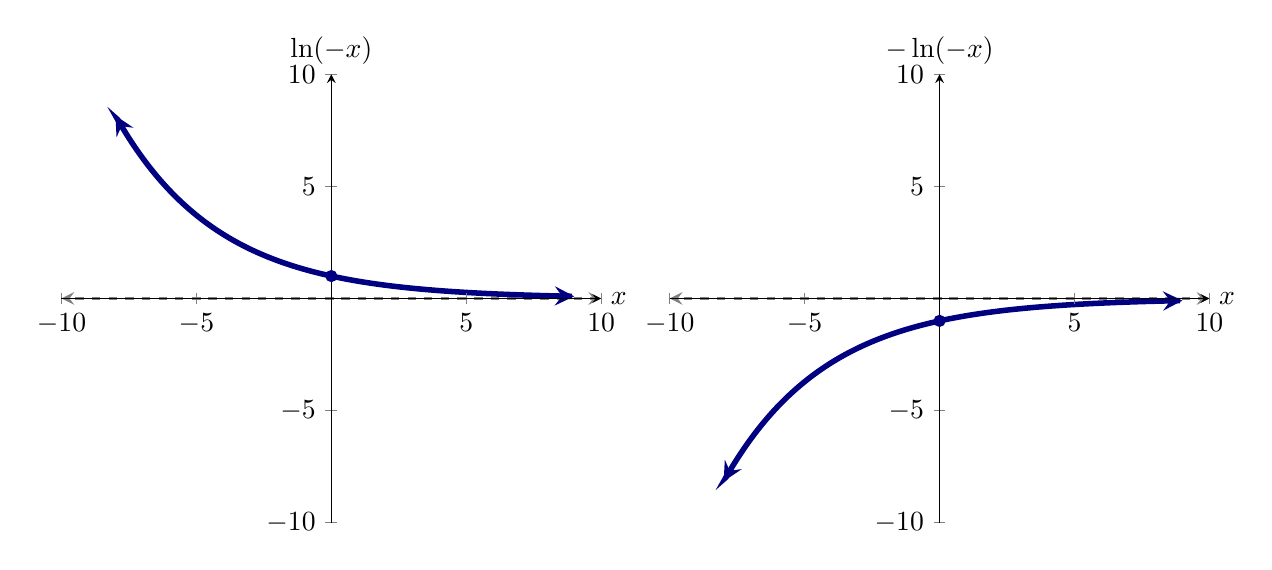
\begin{tikzpicture}
   \begin{axis}[name = leftgraph, 
            domain=-10:10, ymax=10, xmax=10, ymin=-10, xmin=-10,
            axis lines =center, xlabel=$x$, ylabel={$\ln(-x)$},
            every axis y label/.style={at=(current axis.above origin),anchor=south},
            every axis x label/.style={at=(current axis.right of origin),anchor=west},
            axis on top
          ]
          
          \addplot [line width=1, gray, dashed,samples=200,domain=(-10:10),<->] {0};

          \addplot [line width=2, penColor, smooth,samples=200,domain=(-8:9), <->] {1.3^(-x)};
          \addplot [color=penColor,only marks,mark=*] coordinates{(0,1)};
           

  \end{axis}
  \begin{axis}[at={(leftgraph.outer east)},anchor=outer west, 
            domain=-10:10, ymax=10, xmax=10, ymin=-10, xmin=-10,
            axis lines =center, xlabel=$x$, ylabel={$-\ln(-x)$},
            every axis y label/.style={at=(current axis.above origin),anchor=south},
            every axis x label/.style={at=(current axis.right of origin),anchor=west},
            axis on top
          ]
          
          \addplot [line width=1, gray, dashed,samples=200,domain=(-10:10),<->] {0};

          \addplot [line width=2, penColor, smooth,samples=200,domain=(-8:9),<->] {-(1.3^(-x)};
          \addplot [color=penColor,only marks,mark=*] coordinates{(0,-1)};
           

  \end{axis}
\end{tikzpicture}
\end{image}








\subsection*{Pick Your Form}

You should pick your own logarithmic exponential form that you like and understand.  \\

Then, you can change anything given to you into that form.


You might pick a particular number greater than $1$ as the base you like.  $e$ is a very popular choice, because it shows up quite frequently in mathematics, like Calculus. \\











If you pick a base you like and change formulas to use that base, then you have a better chance of quickly deciding on function characteristics. \\



\textbf{\textcolor{blue!55!black}{Basic Basic Form:}}  $\ln(x)$ \\



\textbf{\textcolor{blue!55!black}{Basic Basic Forms:}}  $\ln(x)$, $\ln(-x)$, $-\ln(x)$, $-\ln(-x)$ \\


Now increasing and decreasing become questions about the signs of the two leading coefficents - the leading coefficient of the entire formula and the leading coefficient of the exponent.











\begin{center}
\textbf{\textcolor{green!50!black}{ooooo-=-=-=-ooOoo-=-=-=-ooooo}} \\

more examples can be found by following this link\\ \link[More Examples of Logarithmic Functions]{https://ximera.osu.edu/csccmathematics/precalculus2/precalculus2/logFunctions/examples/exampleList}

\end{center}








\end{document}
